\documentclass[12pt,titlepage]{article}
\usepackage[spanish]{babel}
\usepackage[utf8]{inputenc}
\usepackage[T1]{fontenc}
\usepackage{graphicx}
\usepackage[margin=2cm]{geometry}
\setlength{\parindent}{0mm}

\begin{document} %inicio de documento

\begin{titlepage} %inicio de portada
\begin{center}



\begin{figure}[htbp]
\hspace*{4.0cm} 

\includegraphics[scale=0.25]{Tec_logo}
\end{figure}


\hspace{17mm}\textbf{INSTITUTO TECNOLOGICO JOSÉ MARIO MOLINA \newline
CAMPUS ZAPOPAN}\\[10mm]
 \rule{\linewidth}{1.0mm} 
 \newline
 \uppercase{\\ Miguel ángel pérez bautista}\\[2.5mm]
 \uppercase{ingeniería en electrónica}\\[2.5mm]
 \uppercase{Servomotor Kollmorgen AKM65K}\\[5mm]
 \rule{\linewidth}{1.0mm} 
\end{center}
\end{titlepage}

\section{Servomotores en la industria}
La palabra servomotor no hace referencia a un tipo de motor en concreto sino más bien a un modo de control del motor determinado con el que se consiguen rápidos y muy precisos movimientos. \\

Un servomotor podría ser un motor asíncrono, un motor síncrono, un motor de corriente continua o un motor paso a paso, pero lo que convierte a estos motores en servomotores es el funcionamiento en lazo cerrado.\\

Necesitan un control electrónico de la alimentación y de un detector en el eje que informe al controlador de los valores reales de posición, velocidad y aceleración.\\[0.8mm]

\begin{figure}[!ht]
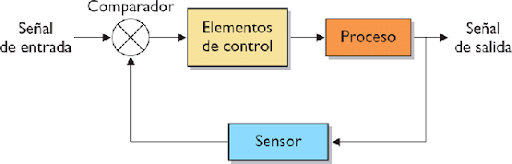
\includegraphics[scale=0.80]{servo1}
\caption{Diagrama de bloques servomotor}
\end{figure}

El controlador electrónico o servodrive trabaja con la modulación de ancho de pulso PWM. 
Con el sistema de funcionamiento en lazo cerrado, el controlador esta continuamente comparando los valores deseados o nominales con los reales medidos con el encoder, en función de la diferencia entre unos y otros aumentará o reducirá la señal enviada. \\[0.8mm] 

Los encoders o resolvers pueden ser absolutos o incrementales. Si bien cada vez es más importante la detección absoluta de posiciones, ya que en muchas aplicaciones no es posible realizar un recorrido de referencia.\\[0.8mm]

Las aplicaciones típicas de los servomotores las encontramos en róbotica, centros de mecanizado por control númerico o procesos de automatización industrial.\\[0.8mm]

\section{Usos de servomotores en industria}
Las aplicaciones de los servomotores en la industria son múltiples y de gran utilidad. Para la industria 4.0 o de la automatización inteligente, el motor servo es un de los instrumentos principales. \\\\
Para las máquinas industriales que están programadas para acciones reptitivas, las aplicaciones de servomotores son muy efectivas. Permiten un mejor control en la producción gracias al control sobre el movimiento del motor.\\[0.8mm]

Las máquinas de grabado en diversos materiales, includias la impresión 3D también se beneficia de las aplicaciones de los servomotores. Para generar diseños complejos, es necesario tener precisión en la ejecución, y el motor servo puede garantizarla.\\[0.8mm]

Un instrumento muy usado en la industria es la máquina de control númerico computarizado, también llamada CNC. Estas máquinas utilizan parámetros exactos para realizar cortes, por lo que necesitan de la ayuda de un motor servo controlable.\\\\

La industria de la robótica también se sirve de las aplicaciones de los servomotores. La robótica en general está siendo utilizada en diversos tipos de manufactura. En sectores como la industria automotriz, hospitalaria y hasta de alimentos, los dispositivos robóticos son de uso constante. \\\\
Los servomotores industriales son esenciales para los nuevos avances en la industria automatizada. Cientos de sectores en pleno crecimiento los utilizan para optimizar procesos y complementar maquinaria especializada. \\\\

Las aplicaciones de este tipo de motores pueden representar una inversión inteligente y ampliamente redituable para dueños de empresas. Es importante considerar su implementación en procesos de manufactura y proyectos de automatización.\\

\section{Servomotor Kollmorgen AKM65K}
Para el desarrollo del proyecto de residencia, donde se está llevado a cabo en el periodo Febrero 2021 a Julio 2021 en CIATEQ Zapopan, se da uso de un servomotor Kollomorgen AKM65K (KM65K-ACCNR-00) para poder realizar movimientos controlados, y a su vez obtener información de interés del  movimiento. 
\paragraph{Servomotor Kollmorgen AKM65K \\}
\hspace{-4.5mm}Un servomotor es un actuador rotativo que permite tener el control preciso de la posición angular. consiste en un motor acomplado a un sensor de posición, para así tener la señal de retroalimentación de posición. Se necesita además del servomotor un servodrive para complementar el sistema. \\\\
La familia de servomotores Kollmorgen te ofrece una opción que jamás se ha visto en el mercado, además de ofrecerte flexibidad en opciones de caracteristicas, para que así puedas implementar al mejor servomotor que se ajuste a tu aplicación. \\\\
Emparejando el servomotor con el servodrive con la familia \textsc{plug and play}, se puede seleccionar los parámetros de control correctos y realizar el movimiento inmediatamente, de una manera fácil nunca antes vista. \\\\

Kollmorgen ofrece una gran variadad de dispositivos estandar, ya sea servomotores o servodrive, ofreciendo lo mejor de ambos. Además si la aplicación requiere de especificaciones especificas, Kollmorgen puede diseñar los dispositivos de acuerdo a los requerimientos de tu aplicación. \\\\

Los servomotores Kollmorgen ofrecen una robustez para poder trabajar en cualquier entorno, ya sea en ambientes calorusos o bajo cero grados, los dispositivos Kollmorgen ofrecen alta calidad de trabajo y desempeño en cualquier entorno de trabajo. \\[25mm]

\begin{figure}[!ht]
\center
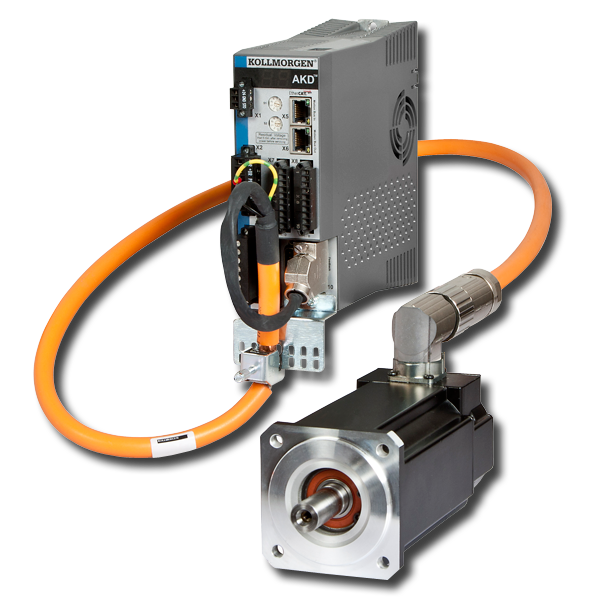
\includegraphics[scale=0.60]{servo2}
\caption{Kollmorgen sistema Servodrive y servomotor}
\end{figure}


 



\end{document}